\begin{infocard}{Proporcionalidad directa}
    Colocaremos en una tabla los 3 datos (a los que llamamos $a$, $b$ y $c$) y
    la incógnita, es decir, el dato que queremos averiguar (que llamaremos
    $x$).
    Después, aplicaremos la siguiente fórmula:
    \begin{center}
        \begin{tabular}{r>{\centering}p{0.2cm}l}
            $a$ & $\Rightarrow$ & $b$ \\
            $c$ & $\Rightarrow$ & $x$
        \end{tabular}\quad$x=\dfrac{c \times b}{a}$
    \end{center}
    % \begin{figure}[H]
    %     \centering
    %     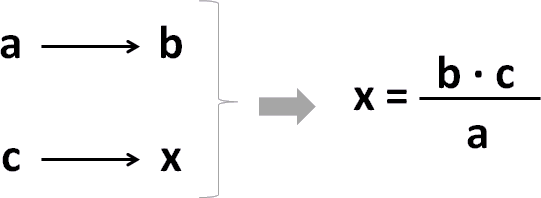
\includegraphics[width=.6\linewidth]{../images/formula-regla-de-3-img1}
    % \end{figure}
\end{infocard}